% Created 2021-10-29 Fri 18:50
% Intended LaTeX compiler: xelatex
\documentclass[12pt]{article}
\usepackage{graphicx}
\usepackage{grffile}
\usepackage{longtable}
\usepackage{wrapfig}
\usepackage{rotating}
\usepackage[normalem]{ulem}
\usepackage{amsmath}
\usepackage{textcomp}
\usepackage{amssymb}
\usepackage{capt-of}
\usepackage{hyperref}
\usepackage{xcolor} % to access the named colour LightGray
\hypersetup{colorlinks,
  filecolor={winered},
  allcolors=.,
  colorlinks=true,
  urlcolor=red!80!black,
  linkcolor=red!80!black,
  filecolor=red!80!black,      
  urlcolor=red!80!black,
  linktoc=page
}
\definecolor{LightGray}{gray}{0.2}
\definecolor{red}{WildStrawberry}{0.2}
\usepackage{minted}
\usemintedstyle{monokai}
\date{\today}
\title{}
\hypersetup{
 pdfauthor={},
 pdftitle={},
 pdfkeywords={},
 pdfsubject={},
 pdfcreator={Emacs 27.2 (Org mode 9.4.4)}, 
 pdflang={English}}

\usepackage{tocloft}
\cftsubsecfont{\color{red}}
\begin{document}

\tableofcontents
\clearpage


\section{Como acessar o conjunto de dados pelo link}
\label{sec:org484c5e1}
Para cada conjunto de dado documentado, há um hyperlink correspondente
pelo qual pode-se acessar o conjunto específico.

{\begin{figure}[!htbp]
    \caption{\href{img/exemplo1.png} Exemplo conjunto gifted.csv}
    \centering
    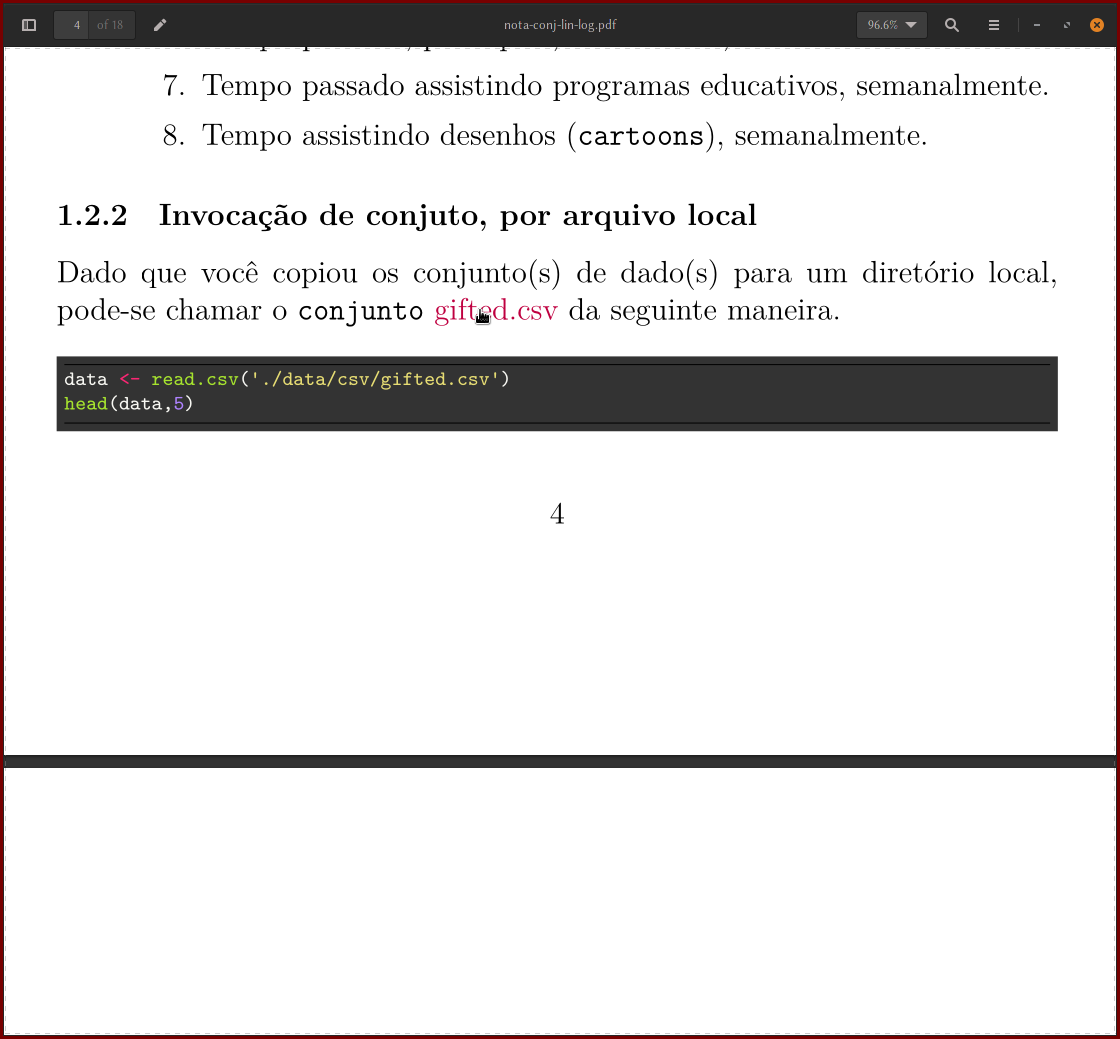
\includegraphics[width=.6\linewidth]{/home/buddhilw/PP/MonitoriaEstatistica/img/exemplo1.png}
\end{figure}}


{\begin{figure}[!htbp]
    \centering
    \caption{\href{img/exemplo2.png}Exemplo direcionamento do hyperlink gifted.csv}
    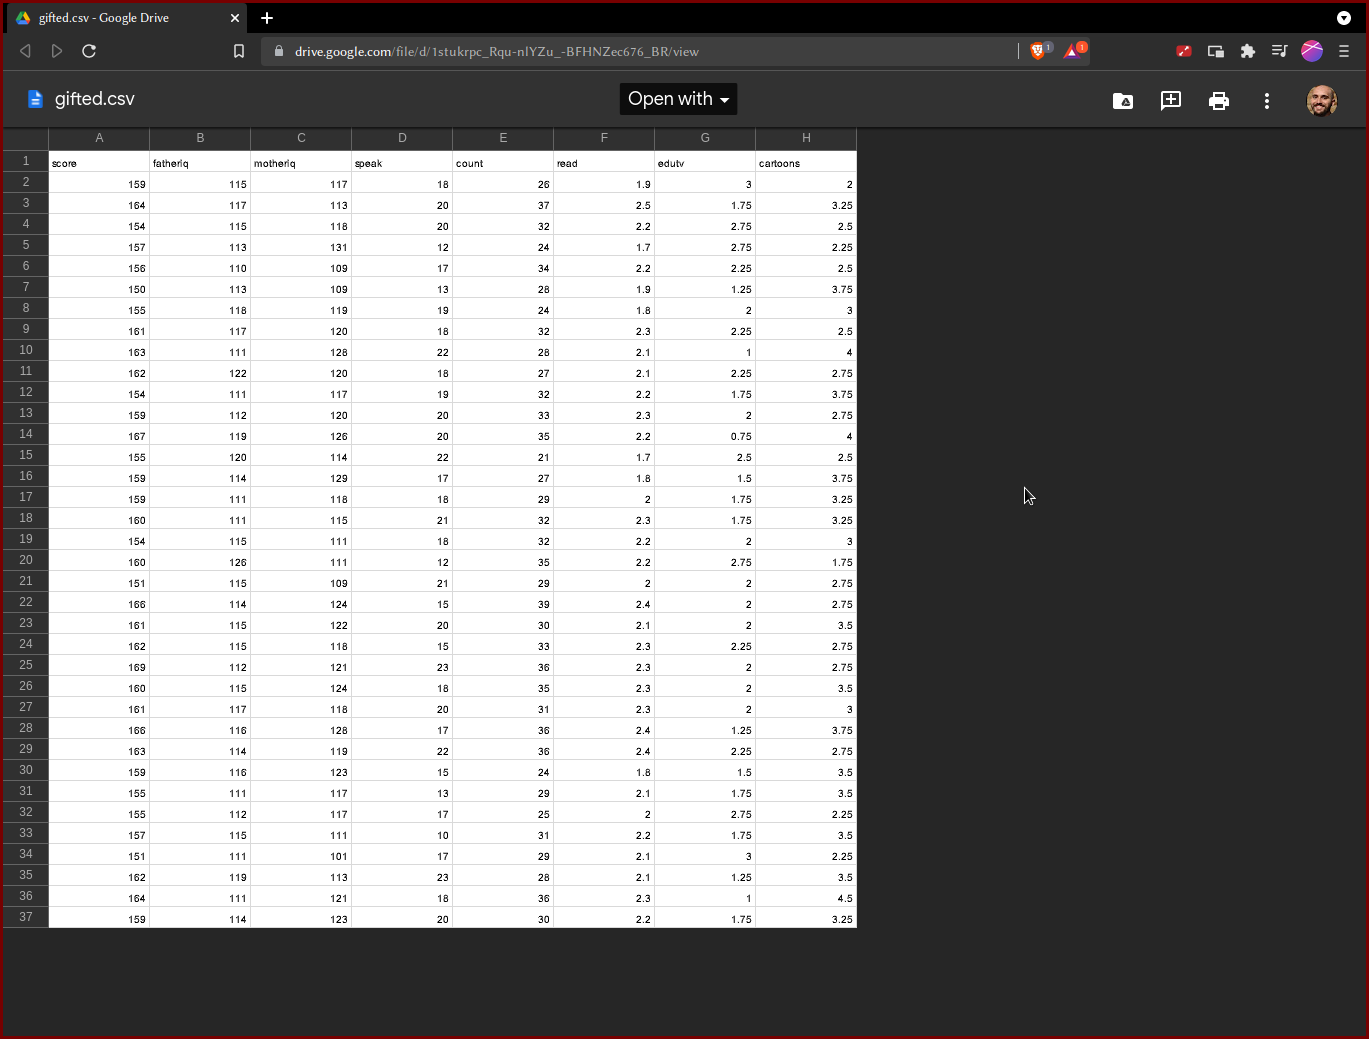
\includegraphics[width=.6\linewidth]{/home/buddhilw/PP/MonitoriaEstatistica/img/exemplo2.png}
\end{figure}}

Ou, acesse os links com todos os dados, e faça o download de todos eles:
\begin{itemize}
\item \href{https://drive.google.com/drive/folders/1SaXLjwvKd\_z6xSQRIs6rxKnOJ7uQguSW?usp=sharing}{Regressão Linear}
\item \href{https://drive.google.com/drive/folders/1BtrKdgg1WzPDfKrSNckv8RcF8DWt-W3F?usp=sharing}{Regressão Logística}
\end{itemize}

E, seguida, siga a secção do documento referente ao conjunto do seu grupo.

\clearpage
\section{Análise de Regressão Linear e Logísticas Múltiplas}
\label{sec:orgd25db30}
\subsection{\href{https://r-data.pmagunia.com/dataset/r-dataset-package-datasets-lifecyclesavings}{Hipótese de ciclos-de-economia salarial}}
\label{sec:orge5e52b7}
\begin{itemize}
\item \textbf{Nome no conjunto de dados:} \href{https://drive.google.com/file/d/1j2K7J1rb3V2Qr\_t0rcBhA6tyuqh88AjY/view?usp=sharing}{savings.csv}
\item \textbf{Variável resposta: \texttt{sr}.}
\item Hipótese formulada por Franco Modigliani 1960-1970, de que essas (outras)
variáveis eram explicativas do fenômeno 'sr'.
\end{itemize}
\subsubsection{Sobre o \texttt{Conjunto}}
\label{sec:orgd10e961}
\begin{itemize}
\item Dados:
\begin{itemize}
\item Sr: valor agregado à economia particular (razão entre valor total de economias pessoais e salário líquido)
\item Pop15: população sob quinze anos de idade.
\item Pop75: população acima de setenta e cinco anos de idade.
\item dpi: valor de salário líquido per-capita médio.
\item ddpi: taxa de crescimento de dpi.
\end{itemize}
\end{itemize}

\subsubsection{Como utilizar pelo R}
\label{sec:orge7010a6}
O \texttt{conjunto de dados} se encontra sob o pacote \texttt{datasets}. Desta forma, precisamos
instalá-lo.

\begin{minted}[frame=lines,fontsize=\scriptsize,linenos=false, bgcolor=LightGray]{r}
install.packages("datasets",mirror="https://vps.fmvz.usp.br/CRAN/")
\end{minted}

Após instalação, precisamos invocar o pacote,
\begin{minted}[frame=lines,fontsize=\scriptsize,linenos=false, bgcolor=LightGray]{r}
library(datasets)
\end{minted}

Finalmente, podemos acessar o \texttt{conjunto},
\begin{minted}[frame=lines,fontsize=\scriptsize,linenos=false, bgcolor=LightGray]{r}
data <- data("LifeCycleSavings")
head(data)
\end{minted}
\subsubsection{Invocação de conjunto, por arquivo local}
\label{sec:org8996014}

Dado que você copiou os conjunto(s) de dado(s) para um diretório
local, pode-se chamar o conjunto \href{https://drive.google.com/file/d/1j2K7J1rb3V2Qr\_t0rcBhA6tyuqh88AjY/view?usp=sharing}{savings.csv} da seguinte maneira.

\begin{minted}[frame=lines,fontsize=\scriptsize,linenos=false, bgcolor=LightGray]{r}
data <- read.csv('./data/csv/savings.csv')
head(data,5)
\end{minted}

\begin{verbatim}
          sr    pop15 pop75 dpi     ddpi
Australia 11.43 29.35 2.87  2329.68 2.87
Austria   12.07 23.32 4.41  1507.99 3.93
Belgium   13.17 23.80 4.43  2108.47 3.82
Bolivia    5.75 41.89 1.67   189.13 0.22
Brazil    12.88 42.19 0.83   728.47 4.56
\end{verbatim}
\clearpage

\subsection{\href{https://www.openintro.org/data/index.php?data=gifted}{Inteligência de prodígios}}
\label{sec:orgb7fdf77}
\begin{itemize}
\item \textbf{Nome no conjunto de dados:} \href{https://drive.google.com/file/d/1stukrpc\_Rqu-nlYZu\_-BFHNZec676\_BR/view?usp=sharing}{gifted.csv}
\item \textbf{Variável resposta: \texttt{score}.}
\end{itemize}
\subsubsection{Sobre o \texttt{Conjunto}}
\label{sec:orgf6db1f7}
\begin{itemize}
\item Referências:
\begin{itemize}
\item Graybill, F.A. \& Iyer, H.K., (1994) Regression Analysis: Concepts and Applications, Duxbury, p. 511-6.
\end{itemize}
\item Dados:
\begin{enumerate}
\item IQ da Criança.
\item IQ Pai.
\item IQ Mãe.
\item Período em meses, até primeiras palavras.
\item Período em meses, até quanto contou até dez.
\item Tempo passado, pelos pais, lendo livros, semanalmente.
\item Tempo passado assistindo programas educativos, semanalmente.
\item Tempo assistindo desenhos (\texttt{cartoons}), semanalmente.
\end{enumerate}
\end{itemize}

\subsubsection{Invocação de conjunto, por arquivo local}
\label{sec:orgee0313e}

Dado que você copiou os conjunto(s) de dado(s) para um diretório
local, pode-se chamar o \texttt{conjunto} \href{https://drive.google.com/file/d/1stukrpc\_Rqu-nlYZu\_-BFHNZec676\_BR/view?usp=sharing}{gifted.csv} da seguinte maneira.

\begin{minted}[frame=lines,fontsize=\scriptsize,linenos=false, bgcolor=LightGray]{r}
data <- read.csv('./data/csv/gifted.csv')
head(data,5)
\end{minted}

\begin{verbatim}
  score fatheriq motheriq speak count read edutv cartoons
1 159   115      117      18    26    1.9  3.00  2.00    
2 164   117      113      20    37    2.5  1.75  3.25    
3 154   115      118      20    32    2.2  2.75  2.50    
4 157   113      131      12    24    1.7  2.75  2.25    
5 156   110      109      17    34    2.2  2.25  2.50    
\end{verbatim}
\clearpage

\subsection{\href{https://www.kaggle.com/augustus0498/life-expectancy-who}{Expectativa de Vida por País}}
\label{sec:org65cf3ae}
\begin{itemize}
\item \textbf{Nome no conjunto de dados:} \href{https://drive.google.com/file/d/1nUnOwgAcWIqoyG0P5\_wnlh1wPxxSUqv5/view}{Life\_Expectancy\_Data.csv}
\item \textbf{Variável resposta: \texttt{Life.expectancy}.}
\end{itemize}
\subsubsection{Sobre o \texttt{Conjunto}}
\label{sec:orgf375ba3}
\begin{itemize}
\item Dados de todos países, derivados da OMS.
\end{itemize}

\begin{itemize}
\item Dados:
\begin{itemize}
\item Country: país,
\item Year: ano correspondente aos dados,
\item Status: estado da industrialização,
\item Life expectancy: expectativa de vida,
\item Adult Mortality \(15<\text{idade}<60\): mortalidade adulta por mil habitantes,
\item Infant deaths: mortalidade infantil por mil habitantes,
\item Alcohol: uso de álcool por litro puro (+15 anos),
\item Percentage expenditure: gasto em saúde em percentagem do PIB per capta,
\item Hepatitis B: percentagem de imunização entre bebês com um ano,
\item Measles: quantidade de casos reportados de Rubeola por mil habitantes,
\item BMI: média de índex de massa corpórea da população,
\item under-five deaths: quantidade de mortes antes dos cinco anos por mil habitantes,
\item Polio: quantidade de imunização entre bebês com um ano (percentagem),
\item Total expenditure: percentagem do gasto total do governo com saúde,
\item Diphtheria: percentagem de imunização de tétano (\(\leq 1 \text{ano}\)),
\item HIV/AIDS: morte a cada mil nascimentos (contanto nascimento de 0-4 anos de idade),
\item GDP: PIB em dólares,
\item Population: População,
\item thinness  1-19 years: prevalência de pessoas magras (1-19 anos de idade),
\item thinness 5-9 years: prevalência de pessoas magras (5-9 anos de idade),
\item Income composition of resources: IDH (qualidade de vida) em termos de composição por salário pessoal (provida por salário próprio),
\item Schooling: média do número de anos sendo educado (escolaridade).
\end{itemize}
\end{itemize}

\subsubsection{Como utilizar o conjunto (cópia de arquivo CSV, localmente)}
\label{sec:orgf6510b3}
Dado que você copiou os conjunto(s) de dado(s) para um diretório
local, pode-se chamar o conjunto \href{https://drive.google.com/file/d/1nUnOwgAcWIqoyG0P5\_wnlh1wPxxSUqv5/view}{Life\_Expectancy\_Data.csv} da seguinte maneira.

Por exemplo, para a análise da expectativa de vida, para o ano de
2015, seria feita invocamos os dados da seguinte maneira,

\begin{minted}[frame=lines,fontsize=\scriptsize,linenos=false, bgcolor=LightGray]{r}
life <- read.csv('./data/csv/Life_Expectancy_Data.csv')
life_2015 <- subset(life, Year=="2015")
life_2015[1:6,1:5] 
\end{minted}

\begin{verbatim}
   Country             Year Status     Life.expectancy Adult.Mortality
1  Afghanistan         2015 Developing 65.0            263            
17 Albania             2015 Developing 77.8             74            
33 Algeria             2015 Developing 75.6             19            
49 Angola              2015 Developing 52.4            335            
65 Antigua and Barbuda 2015 Developing 76.4             13            
81 Argentina           2015 Developing 76.3            116            
\end{verbatim}


Obs: apenas 5 colunas foram selecionadas, por motivos estéticos na formatação.
\clearpage

\subsection{\href{https://www.sheffield.ac.uk/mash/statistics/datasets}{Peso ao Nascimento}}
\label{sec:orgde1797d}
\begin{itemize}
\item \textbf{Nome no conjunto de dados:} \href{https://drive.google.com/file/d/1xv2lCPsj04FjGPQ\_BgPS9mrTIjBcyHQk/view?usp=sharing}{Birth Weight}
\item \textbf{Variável resposta: \texttt{Birthweight}.}.
\end{itemize}
\subsubsection{Dados sobre o \texttt{Conjunto}}
\label{sec:orgcabc7ec}
\begin{itemize}
\item Dados:
\begin{itemize}
\item lowbwt: baixo peso ao nascer.
\item ID: Identificador
\item mage35: mãe mais velha do que 35 anos.
\item fnocig: número de cigarros fumado pelo pai diariamente.
\item fheight: peso do pai (kg)
\item fedyrs: quantidade de anos de educação do pai
\item fage: idade do pai
\item mppwt: peso da mãe pré gravidez.
\item mheight: tamanho da mãe (cm).
\item mnocig: número de cigarros fumados diariamente pela mãe.
\item Motherage: idade da mãe.
\item Gestation Smoker: fumante durante gestação
\item headcirumfer: circunferência da cabeça
\item length: tamanho (cm)
\end{itemize}
\end{itemize}
\subsubsection{Invocação de conjuto, por arquivo local}
\label{sec:org9855019}

Dado que você copiou os conjunto(s) de dado(s) para um diretório
local, pode-se chamar o conjunto \href{https://drive.google.com/file/d/1xv2lCPsj04FjGPQ\_BgPS9mrTIjBcyHQk/view?usp=sharing}{Birth Weight} da seguinte maneira.

\begin{minted}[frame=lines,fontsize=\scriptsize,linenos=false, bgcolor=LightGray]{r}
data <- read.csv('./data/csv/Birthweight_reduced_kg_R.csv')
head(data,5)
\end{minted}

\begin{verbatim}
  X...ID Length Birthweight Headcirc Gestation smoker mage mnocig mheight mppwt
1 1360   56     4.55        34       44        0      20   0      162     57   
2 1016   53     4.32        36       40        0      19   0      171     62   
3  462   58     4.10        39       41        0      35   0      172     58   
4 1187   53     4.07        38       44        0      20   0      174     68   
5  553   54     3.94        37       42        0      24   0      175     66   
  fage fedyrs fnocig fheight lowbwt mage35
1 23   10     35     179     0      0     
2 19   12      0     183     0      0     
3 31   16     25     185     0      1     
4 26   14     25     189     0      0     
5 30   12      0     184     0      0     
\end{verbatim}
\clearpage

\subsection{\href{https://www.sheffield.ac.uk/mash/statistics/datasets}{Crime}}
\label{sec:orgbab30bb}
\begin{itemize}
\item \textbf{Nome no conjunto de dados:} \href{https://drive.google.com/file/d/1hZpHoEXbhZGvmtmrbcWpXYfBV-2ZD7uF/view?usp=sharing}{Crimes}
\item \textbf{Variável resposta: \texttt{CrimeRate}.}.
\end{itemize}
\subsubsection{Dados sobre o \texttt{Conjunto}}
\label{sec:orgb5f5338}
\begin{itemize}
\item Dados:
\begin{itemize}
\item CrimeRate: Taxa de criminalidade (ofensas por milhão de habitantes).
\item Youth: Jovens entre 18-24 anos a cada mil habitantes.
\item Southern: Estado do sul?
\item Education: Tempo de educação (anos de estudo até 25)
\item ExpenditureYear0: Dinheiro para segurança pública per capta.
\item LabourForce: Quantidade de jovens trabalhadores por 1000 habitantes.
\item Males: Homens (por cada 1000 mulheres).
\item MoreMales: Mais homens que mulheres?.
\item StateSize: Tamanho do estado em milhares.
\item YouthUnemployment: Desemprego de jovens por mil.
\item BelowWage: Número de famílias abaixo de meio salário por mil.
\item Wage: Salário médio semanal.
\item MatureUnemployment: Desemprego de sêniores (35-39) por mil.
\end{itemize}
\end{itemize}

\subsubsection{Invocação de conjuto, por arquivo local}
\label{sec:org698e03f}

Dado que você copiou os conjunto(s) de dado(s) para um diretório
local, pode-se chamar o conjunto \href{https://drive.google.com/file/d/1hZpHoEXbhZGvmtmrbcWpXYfBV-2ZD7uF/view?usp=sharing}{Crimes} da seguinte maneira.

\begin{minted}[frame=lines,fontsize=\scriptsize,linenos=false, bgcolor=LightGray]{r}
data <- read.csv('./data/csv/Crime_R.csv')
head(data,5)
\end{minted}

\begin{verbatim}
  X...CrimeRate Youth Southern Education ExpenditureYear0 LabourForce Males
1 45.5          135   0        12.4       69              540          965 
2 52.3          140   0        10.9       55              535         1045 
3 56.6          157   1        11.2       47              512          962 
4 60.3          139   1        11.9       46              480          968 
5 64.2          126   0        12.2      106              599          989 
  MoreMales StateSize YouthUnemployment ... ExpenditureYear10 LabourForce10
1 0          6         80               ... 71                564          
2 1          6        135               ... 54                540          
3 0         22         97               ... 44                529          
4 0         19        135               ... 41                497          
5 0         40         78               ... 97                602          
  Males10 MoreMales10 StateSize10 YouthUnemploy10 MatureUnemploy10
1  974    0            6           82             20              
2 1039    1            7          138             39              
3  959    0           24           98             33              
4  983    0           20          131             50              
5  989    0           42           79             24              
  HighYouthUnemploy10 Wage10 BelowWage10
1 1                   632    142        
2 1                   521    210        
3 0                   359    256        
4 0                   510    235        
5 1                   660    162        
\end{verbatim}
\clearpage

\subsection{\href{https://r-data.pmagunia.com/dataset/r-dataset-package-datasets-attitude}{Atitudes em relação à empresa}}
\label{sec:org7675ac9}
\begin{itemize}
\item \textbf{Nome no conjunto de dados:} \href{https://drive.google.com/file/d/1rKj4NPD61bWKD6HBC4fux2Eit6CNEKwr/view?usp=sharing}{Atitude}
\item \textbf{Variável resposta: \texttt{rating}.}
\end{itemize}
\subsubsection{Sobre o \texttt{Conjunto}}
\label{sec:org1e5b938}
\begin{itemize}
\item Dados: (em percentagem)
\begin{itemize}
\item Complaints: percentagem de resoluções de reclamações.
\item Privileges: percentagem de intolerância de privilégios.
\item Learning: percentagem de oportunidade de aprendizado.
\item Raises: percetagem de aumento correspondente à performance.
\item Critical: percentagem de atitudes e críticas exacerbadas.
\item Advancel: percentagem de evolução percebida da empresa e posto.
\item Rating: avaliação geral positiva da empresa
\end{itemize}
\end{itemize}

\subsubsection{Como utilizar pelo R}
\label{sec:orgc310b70}
O \texttt{conjunto de dados} se encontra sob o pacote \texttt{datasets}. Desta forma, precisamos
instalá-lo.

\begin{minted}[frame=lines,fontsize=\scriptsize,linenos=false, bgcolor=LightGray]{r}
install.packages("datasets",mirror="https://vps.fmvz.usp.br/CRAN/")
\end{minted}

Após instalação, precisamos invocar o pacote,
\begin{minted}[frame=lines,fontsize=\scriptsize,linenos=false, bgcolor=LightGray]{r}
library(datasets)
\end{minted}

Finalmente, podemos acessar o \texttt{conjunto},
\begin{minted}[frame=lines,fontsize=\scriptsize,linenos=false, bgcolor=LightGray]{r}
data <- data("attitude")
head(data)
\end{minted}
\subsubsection{Invocação de conjuto, por arquivo local}
\label{sec:orgb9dad86}

Dado que você copiou os conjunto(s) de dado(s) para um diretório
local, pode-se chamar o conjunto \href{https://drive.google.com/file/d/1rKj4NPD61bWKD6HBC4fux2Eit6CNEKwr/view?usp=sharing}{Atitude} da seguinte maneira.

\begin{minted}[frame=lines,fontsize=\scriptsize,linenos=false, bgcolor=LightGray]{r}
data <- read.csv('./data/csv/attitude.csv')
head(data,5)
\end{minted}

\begin{verbatim}
  rating complaints privileges learning raises critical advance
1 43     51         30         39       61     92       45     
2 63     64         51         54       63     73       47     
3 71     70         68         69       76     86       48     
4 61     63         45         47       54     84       35     
5 81     78         56         66       71     83       47     
\end{verbatim}
\clearpage

\subsection{\href{https://archive.ics.uci.edu/ml/datasets/Breast+Cancer+Wisconsin+\%28Diagnostic\%29}{Câncer de Mama}}
\label{sec:org92d804a}
\begin{itemize}
\item \textbf{Nome no conjunto de dados:} \href{https://drive.google.com/file/d/14WFx8oXCYst\_QPySIfuii660A93xg4pg/view?usp=sharing}{wdbc.data}
\item \textbf{Variável resposta:  \texttt{Diagnosis}.}
\end{itemize}
\subsubsection{Sobre o \texttt{Conjunto}}
\label{sec:org06eb3b0}
\begin{itemize}
\item Dados:
\begin{enumerate}
\item Número Identificador (ID).
\item Diagnóstico (M=maligno, B=belígero).
\item Dez variáveis contínuas reais, com três medidas, médias, erro e pior medida (maiores valores)
\begin{enumerate}
\item Raio da mancha
\item Textura
\item Perímetro
\item Área
\item Suavidade
\item Compactividade (Quão compacto)
\item Concavidade
\item Pontos de Concavidade
\item Simetria
\item Dimensão Fractal (formato das bordas)
\end{enumerate}
\end{enumerate}
\end{itemize}
\subsubsection{Invocação de conjuto, por arquivo local}
\label{sec:orgcc0e41d}

Dado que você copiou os conjunto(s) de dado(s) para um diretório
local, pode-se chamar o \texttt{conjunto} \href{https://drive.google.com/file/d/14WFx8oXCYst\_QPySIfuii660A93xg4pg/view?usp=sharing}{wdbc.data} da seguinte maneira.

\begin{minted}[frame=lines,fontsize=\scriptsize,linenos=false, bgcolor=LightGray]{r}
data <- read.csv('./data/csv/wdbc.data')
head(data,5)
\end{minted}

\begin{verbatim}
  ID       Diagnosis Radius.mean Texture.mean Perimeter.mean Area.mean
1   842302 M         17.99       10.38        122.80         1001.0   
2   842517 M         20.57       17.77        132.90         1326.0   
3 84300903 M         19.69       21.25        130.00         1203.0   
4 84348301 M         11.42       20.38         77.58          386.1   
5 84358402 M         20.29       14.34        135.10         1297.0   
  Smoothness.mean Compactness.mean Concavity.mean Concavity.poits.mean ...
1 0.11840         0.27760          0.3001         0.14710              ...
2 0.08474         0.07864          0.0869         0.07017              ...
3 0.10960         0.15990          0.1974         0.12790              ...
4 0.14250         0.28390          0.2414         0.10520              ...
5 0.10030         0.13280          0.1980         0.10430              ...
  Radius.worst Texture.worst Perimeter.worst Area.worst Smoothness.worst
1 25.38        17.33         184.60          2019.0     0.1622          
2 24.99        23.41         158.80          1956.0     0.1238          
3 23.57        25.53         152.50          1709.0     0.1444          
4 14.91        26.50          98.87           567.7     0.2098          
5 22.54        16.67         152.20          1575.0     0.1374          
  Compactness.worst Concavity.worst Concavity.poits.worst Symmetry.worst
1 0.6656            0.7119          0.2654                0.4601        
2 0.1866            0.2416          0.1860                0.2750        
3 0.4245            0.4504          0.2430                0.3613        
4 0.8663            0.6869          0.2575                0.6638        
5 0.2050            0.4000          0.1625                0.2364        
  Fractal.dim.worst
1 0.11890          
2 0.08902          
3 0.08758          
4 0.17300          
5 0.07678          
\end{verbatim}
\clearpage

\subsection{\href{https://www.kaggle.com/uciml/pima-indians-diabetes-database}{Diabetes}}
\label{sec:orgc90c655}
\begin{itemize}
\item \textbf{Nome no conjunto de dados:} \href{https://drive.google.com/file/d/19eaULwopwE1hco\_R9QZIXqDuA3CS2OBh/view?usp=sharing}{diabetes.csv}
\item \textbf{Variável resposta:  \texttt{Outcome}.}
\end{itemize}
\subsubsection{Sobre o \texttt{Conjunto}}
\label{sec:org57088c6}
\begin{itemize}
\item Dados:
\begin{enumerate}
\item Pregnancies: número de gravidezes.
\item Glucose: concentração de glucose durante teste.
\item BloodPressure: pressão sanguínea.
\item SkinThickness: espessura da pele.
\item Insulin: nível de insulina
\item BMI: índex de massa corporal.
\item DiabetesPedigreeFunction: valor da função modelando hereditariedade.
\item Age: idade.
\item Outcome: tem (1) ou não (0) diabetes.
\end{enumerate}
\end{itemize}
\subsubsection{Invocação de conjuto, por arquivo local}
\label{sec:org036aff5}

Dado que você copiou os conjunto(s) de dado(s) para um diretório
local, pode-se chamar o \texttt{conjunto} \href{https://drive.google.com/file/d/19eaULwopwE1hco\_R9QZIXqDuA3CS2OBh/view?usp=sharing}{diabetes.csv} da seguinte maneira.

\begin{minted}[frame=lines,fontsize=\scriptsize,linenos=false, bgcolor=LightGray]{r}
data <- read.csv('./data/csv/diabetes.csv')
head(data,5)
\end{minted}

\begin{verbatim}
  Pregnancies Glucose BloodPressure SkinThickness Insulin BMI 
1 6           148     72            35              0     33.6
2 1            85     66            29              0     26.6
3 8           183     64             0              0     23.3
4 1            89     66            23             94     28.1
5 0           137     40            35            168     43.1
  DiabetesPedigreeFunction Age Outcome
1 0.627                    50  1      
2 0.351                    31  0      
3 0.672                    32  1      
4 0.167                    21  0      
5 2.288                    33  1      
\end{verbatim}
\clearpage

\subsection{\href{https://archive.ics.uci.edu/ml/datasets/Rice+\%28Cammeo+and+Osmancik\%29}{Arrozal}}
\label{sec:org59d8608}
\begin{itemize}
\item \textbf{Nome no conjunto de dados:}  \href{https://drive.google.com/file/d/1zFkHbui6Ro2N\_tNsgPSeajyl7g8XrdAc/view?usp=sharing}{rice.csv}
\item \textbf{Variável resposta:  \texttt{Class}.}
\end{itemize}
\subsubsection{Sobre o \texttt{Conjunto}}
\label{sec:orgf3a8a16}
\begin{itemize}
\item Dados:
\begin{enumerate}
\item Area: área.
\item Perimeter: perímetro.
\item Major.Axis: eixo majoritário.
\item Minor.Axis: eixo minoritário.
\item Eccentricity: excentricidade.
\item Convex.Area: area convexa.
\item Extent: extensão.
\item Class: Cammeo ou Osmancik (qual arrozal?)
\end{enumerate}
\end{itemize}
\subsubsection{Invocação de conjuto, por arquivo local}
\label{sec:orga5d35e9}

Dado que você copiou os conjunto(s) de dado(s) para um diretório
local, pode-se chamar o \texttt{conjunto} \href{https://drive.google.com/file/d/1zFkHbui6Ro2N\_tNsgPSeajyl7g8XrdAc/view?usp=sharing}{rice.csv} da seguinte maneira.

\begin{minted}[frame=lines,fontsize=\scriptsize,linenos=false, bgcolor=LightGray]{r}
data <- read.csv('./data/csv/rice.csv')
head(data,5)
\end{minted}

\begin{verbatim}
  Area  Perimeter Major.Axis Minor.Axis Eccentricity Convex.Area Extent   
1 15231 525.579   229.7499   85.09379   0.9288820    15617       0.5728955
2 14656 494.311   206.0201   91.73097   0.8954050    15072       0.6154363
3 14634 501.122   214.1068   87.76829   0.9121181    14954       0.6932588
4 13176 458.343   193.3374   87.44839   0.8918609    13368       0.6406690
5 14688 507.167   211.7434   89.31245   0.9066909    15262       0.6460239
  Class 
1 Cammeo
2 Cammeo
3 Cammeo
4 Cammeo
5 Cammeo
\end{verbatim}
\clearpage

\subsection{\href{https://archive.ics.uci.edu/ml/datasets/Algerian+Forest+Fires+Dataset++}{Queimadas em Florestas}}
\label{sec:orga494250}
\begin{itemize}
\item \textbf{Nome no conjunto de dados:} \href{https://drive.google.com/file/d/1zuMrZgUo9vRH80HA7zJiBRJpBkGBw3hb/view?usp=sharing}{forest.csv}
\item \textbf{Variável resposta:  \texttt{Classes}.}
\end{itemize}
\subsubsection{Sobre o \texttt{Conjunto}}
\label{sec:orga9a8717}
\begin{itemize}
\item Dados:
\begin{enumerate}
\item day: dia.
\item month: mês.
\item year: ano.
\item Temperature: temperatura.
\item RH: umidade relativa.
\item Ws: velocidade do vento.
\item Rain: total do dia em mm.
\item FFMC: índice de quão inflamável estava a matéria orgânica (Fine fuel moisture code).
\item DMC: índide de quão inflamável estava materiais em decomposição (Duff moisture code).
\item DC: índice de quão árido/seco.
\item ISI: índice de dispersão inicial.
\item BUI: índice de velocidade de dispersão.
\item FWI: índice de clima propício à queimada.
\item Classes: houve ou não queimada.
\end{enumerate}
\end{itemize}

\subsubsection{Invocação de conjuto, por arquivo local}
\label{sec:org82ad133}

Dado que você copiou os conjunto(s) de dado(s) para um diretório
local, pode-se chamar o \texttt{conjunto} \href{https://drive.google.com/file/d/1zuMrZgUo9vRH80HA7zJiBRJpBkGBw3hb/view?usp=sharing}{forest.csv} da seguinte maneira.

\begin{minted}[frame=lines,fontsize=\scriptsize,linenos=false, bgcolor=LightGray]{r}
data <- read.csv('./data/csv/forest.csv')
head(data,5)
\end{minted}

\begin{verbatim}
  day month year Temperature RH Ws Rain FFMC DMC DC   ISI BUI FWI Classes    
1 01  06    2012 29          57 18 0    65.7 3.4 7.6  1.3 3.4 0.5 not fire   
2 02  06    2012 29          61 13 1.3  64.4 4.1 7.6  1   3.9 0.4 not fire   
3 03  06    2012 26          82 22 13.1 47.1 2.5 7.1  0.3 2.7 0.1 not fire   
4 04  06    2012 25          89 13 2.5  28.6 1.3 6.9  0   1.7 0   not fire   
5 05  06    2012 27          77 16 0    64.8 3   14.2 1.2 3.9 0.5 not fire   
\end{verbatim}
\clearpage

\subsection{\href{https://archive.ics.uci.edu/ml/datasets/Contraceptive+Method+Choice}{Método Contraceptivo}}
\label{sec:org57eb7d3}
\begin{itemize}
\item \textbf{Nome no conjunto de dados:} \href{https://drive.google.com/file/d/1M774v2s0uxQorn7w-ASPOfpPoAb93I2m/view?usp=sharing}{cmc.data}
\item \textbf{Variável resposta:  \texttt{Contraceptive.method}.}
\end{itemize}
\begin{enumerate}
\item Sobre o \texttt{Conjunto}
\label{sec:org9d9ddef}
\begin{itemize}
\item Dados:
\begin{enumerate}
\item Wife.age: idade da esposa.
\item Wife.edu: educação esposa.
\item Husband.edu: educação marido.
\item Children.num: número de filhos.
\item Wife.religion: religião esposa.
\item Wife.NotWorking.stat: status da esposa, não trabalhando (1) ou trabalhando (0).
\item Husband.occupation: ocupação do marido.
\item Standard.living: qualidade de vida.
\item Media.exposure: exposição à mídia.
\item Contraceptive.method: método contraceptivo.
\end{enumerate}
\end{itemize}
\end{enumerate}

\subsubsection{Invocação de conjuto, por arquivo local}
\label{sec:orgc54fb90}

Dado que você copiou os conjunto(s) de dado(s) para um diretório
local, pode-se chamar o \texttt{conjunto} \href{https://drive.google.com/file/d/1M774v2s0uxQorn7w-ASPOfpPoAb93I2m/view?usp=sharing}{cmc.data} da seguinte maneira.

\begin{minted}[frame=lines,fontsize=\scriptsize,linenos=false, bgcolor=LightGray]{r}
data <- read.csv('./data/csv/cmc.data')
head(data,5)
\end{minted}

\begin{verbatim}
  Wife.age Wife.edu Husband.edu Children.num Wife.religion Wife.NotWorking.stat
1 24       2        3            3           1             1                   
2 45       1        3           10           1             1                   
3 43       2        3            7           1             1                   
4 42       3        2            9           1             1                   
5 36       3        3            8           1             1                   
  Husband.occupation Standard.living Media.exposure Contraceptive.method
1 2                  3               0              1                   
2 3                  4               0              1                   
3 3                  4               0              1                   
4 3                  3               0              1                   
5 3                  2               0              1                   
\end{verbatim}
\clearpage

\subsection{\href{https://archive.ics.uci.edu/ml/datasets/Thoracic+Surgery+Data}{Cirurgia Torácica}}
\label{sec:orgd485175}
\begin{itemize}
\item \textbf{Nome no conjunto de dados:} \href{https://drive.google.com/file/d/13s1ZtCWotN\_VwQb07yTWEyBMmvO042At/view?usp=sharing}{ThoraicSurgery.csv}
\item \textbf{Variável resposta:  \texttt{Risk1Yr}.}
\end{itemize}
\subsubsection{Sobre o \texttt{Conjunto}}
\label{sec:orgadf5328}
\begin{itemize}
\item Dados:
\begin{enumerate}
\item DNG: combinações específicas de códigos genéticos ativos,
\item PRE4: capacidade vital forçada (FVC),
\item PRE5: volume expirado,
\item PRE6: status da performance (escala de  Zubrod),
\item PRE7: dor anterior à cirurgia,
\item PRE8: hematopoese anterior à cirurgia,
\item PRE9: dispneia anterior à cirurgia,
\item PRE10: toce anterior à cirurgia,
\item PRE11: fraqueza anterior à cirurgia,
\item PRE14: tamanho inidial do tumor,
\item PRE17: presença de diabete tipo 2,
\item PRE19: infarto do miocárdio seis meses antes da cirurgia,
\item PRE25: presença de doenças arterial periférica,
\item PRE30: fumante,
\item PRE32: asma,
\item AGE: idade quando fez cirurgia,
\item Risk1Yr: período de menos de um ano de sobrevivência após cirurgia (T=morte, F=continuou vivo),
\end{enumerate}
\end{itemize}

\subsubsection{Invocação de conjuto, por arquivo local}
\label{sec:org13134a6}

Dado que você copiou os conjunto(s) de dado(s) para um diretório
local, pode-se chamar o \texttt{conjunto} \href{https://drive.google.com/file/d/13s1ZtCWotN\_VwQb07yTWEyBMmvO042At/view?usp=sharing}{ThoraicSurgery.csv} da seguinte maneira.

\begin{minted}[frame=lines,fontsize=\scriptsize,linenos=false, bgcolor=LightGray]{r}
data <- read.csv('./data/csv/ThoraricSurgery.csv')
head(data,5)
\end{minted}

\begin{verbatim}
  DNG  PRE4 PRE5 PRE6 PRE7  PRE8  PRE9  PRE10 PRE11 PRE14 PRE17 PRE19 PRE25
1 DGN2 2.88 2.16 PRZ1 FALSE FALSE FALSE  TRUE  TRUE OC14  FALSE FALSE FALSE
2 DGN3 3.40 1.88 PRZ0 FALSE FALSE FALSE FALSE FALSE OC12  FALSE FALSE FALSE
3 DGN3 2.76 2.08 PRZ1 FALSE FALSE FALSE  TRUE FALSE OC11  FALSE FALSE FALSE
4 DGN3 3.68 3.04 PRZ0 FALSE FALSE FALSE FALSE FALSE OC11  FALSE FALSE FALSE
5 DGN3 2.44 0.96 PRZ2 FALSE  TRUE FALSE  TRUE  TRUE OC11  FALSE FALSE FALSE
  PRE30 PRE32 AGE Risk1Yr
1  TRUE FALSE 60  FALSE  
2  TRUE FALSE 51  FALSE  
3  TRUE FALSE 59  FALSE  
4 FALSE FALSE 54  FALSE  
5  TRUE FALSE 73   TRUE  
\end{verbatim}
\end{document}